\documentclass[11pt]{article}
\usepackage{fullpage,fourier,amsmath,amssymb}
\usepackage{listings,color,url,hyperref}
\usepackage{graphicx}
\usepackage{mdframed}
\usepackage{wrapfig}
\usepackage{epigraph}
\usepackage[x11names]{xcolor}

\title{Assignment 6 \\ Huffman Coding}
\author{Prof. Darrell Long \\ CSE 13S -- Spring 2021}
\date{
  First \texttt{DESIGN.pdf} draft due: May 13$^\text{th}$ at 11:59\,pm PST \\
  Assignment due: May 23$^\text{rd}$ at 11:59\,pm PST
}

\usepackage{fancyhdr}
\pagestyle{fancy}
\fancyhf{}

\fancypagestyle{plain}{%
  \fancyhf{}
  \renewcommand{\headrulewidth}{0pt}
  \renewcommand{\footrulewidth}{0pt}
  \lfoot{\textcopyright{} 2021 Darrell Long}
  \rfoot{\thepage}
}

\pagestyle{plain}

\definecolor{codegreen}{rgb}{0,0.5,0}
\definecolor{codegray}{rgb}{0.5,0.5,0.5}
\definecolor{codepurple}{rgb}{0.58,0,0.82}

\lstloadlanguages{C,make,python,fortran}

\lstdefinestyle{c99}{
    morekeywords={bool, uint8_t, uint16_t, uint32_t, uint64_t, int8_t, int16_t, int32_t, int64_t},
    commentstyle=\color{codegreen},
    keywordstyle=\color{magenta},
    numberstyle=\tiny\color{codegray},
    identifierstyle=\color{blue},
    stringstyle=\color{codepurple},
    basicstyle=\ttfamily,
    breakatwhitespace=false,
    breaklines=true,
    captionpos=b,
    keepspaces=true,
    numbers=left,
    numbersep=5pt,
    showspaces=false,
    showstringspaces=false,
    showtabs=false,
    tabsize=4
}


\begin{document}\maketitle

\section{Introduction}

\epigraphwidth=0.618034\textwidth
\epigraph{\emph{You're trying to take something that can be described in
many, many sentences and pages of prose, but you can convert it into a couple
lines of poetry and you still get the essence, so that's compression.
The best code is poetry.}}{---Satya Nadella}

\begin{wrapfigure}{r}{0.2\textwidth}
  \begin{center}
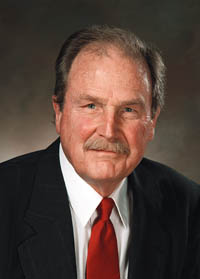
\includegraphics[width=0.15\textwidth]{images/huffman.jpg}
\centerline{\small David A. Huffman}
  \end{center}
\end{wrapfigure}

When David Huffman was a graduate student in a class at MIT, the
professor gave the class an unsolved problem: How to construct an
optimal static encoding of information. The young Huffman came back
a few days later with his solution, and that solution changed the
world. Data compression is now used in all aspects of communication.
David Huffman joined the faculty of MIT in 1953, and in 1967 he
joined the faculty of University of California, Santa Cruz as one
of its earliest members and helped to found its Computer Science
Department, where he served as chairman from 1970 to 1973. He retired
in 1994, and passed away in 1999.

The key idea is called \emph{entropy}, originally defined by Claude Shannon in
1948. Entropy is a measure of the amount of information in a, say, set of
symbols. If we define $I(x) = \log_2 \Pr[x]$ to be the information content of
a symbol, then the entropy of the set $X=\{x_1, \ldots, x_n \}$ is
$$
H(X) = \sum_{i=1}^n \Pr[x_i] I(x_i) = - \sum_{i=1}^n \Pr[x_i] \log_2 \Pr[x_i].
$$
It should be easy to see that the optimal \emph{static} encoding will assign
the least number of \emph{bits} to the most common symbol, and the greatest
number of bits to the least common symbol.

\section{The Encoder}

Your first task for this assignment is to implement a Huffman encoder.
This encoder will read in an input file, find the Huffman encoding of
its contents, and use the encoding to compress the file. Your encoder
program, named \texttt{encode}, must support any combination of the
following command-line options:

\begin{itemize}
  \item \textbf{\texttt{-h}}\,: Prints out a help message describing the purpose
    of the program and the command-line options it accepts, exiting the
    program afterwards. Refer to the reference program in the resources
    repo for an idea of what to print.

  \item \textbf{\texttt{-i infile}}\,: Specifies the input file to encode using
    Huffman coding. The default input should be set as \texttt{stdin}.

  \item \textbf{\texttt{-o outfile}}\,: Specifies the output file to
    write the compressed input to. The default output should be set as
    \texttt{stdout}.

  \item \textbf{\texttt{-v}}\,: Prints compression statistics to
    \texttt{stderr}. These statistics include the uncompressed file
    size, the compressed file size, and \emph{space saving}. The formula
    for calculating space saving is:
    \[
        100 \times (1 - (\text{compressed size} / \text{uncompressed
        size})).
    \]
    Refer to the reference program in the resources repository for the
    exact output.
\end{itemize}

\noindent The algorithm to encode a file, or to compress it, is as follows:

\begin{enumerate}
  \item Compute a histogram of the file. In other words, count the
    number of occurrences of each unique symbol in the file.

  \item Construct the Huffman tree using the computed histogram. This
    will require a \emph{priority queue}.

  \item Construct a code table. Each index of the table represents a
    symbol and the value at that index the symbol's code. You will need
    to use a \emph{stack of bits} and perform a traversal of the Huffman
    tree.

  \item Emit an encoding of the Huffman tree to a file. This will be
    done through a \emph{post-order traversal} of the Huffman tree. The
    encoding of the Huffman tree will be referred to as a \emph{tree
    dump}.

  \item Step through each symbol of the input file again. For each
    symbol, emit its code to the output file.
\end{enumerate}

\section{The Decoder}

The second task for this assignment is to implement a Huffman decoder.
This decoder will read in a compressed input file and decompress it,
expanding it back to its original, uncompressed size. Your decoder
program, named \texttt{decode}, must support any combination of the
following command-line options.

\begin{itemize}
  \item \textbf{\texttt{-h}}\,: Prints out a help message describing the purpose
    of the program and the command-line options it accepts, exiting the
    program afterwards. Refer to the reference program in the resources
    repo for an idea of what to print.

  \item \textbf{\texttt{-i infile}}\,: Specifies the input file to
    decode using Huffman coding. The default input should be set as
    \texttt{stdin}.

  \item \textbf{\texttt{-o outfile}}\,: Specifies the output file to
    write the decompressed input to. The default output should be set as
    \texttt{stdout}.

  \item \textbf{\texttt{-v}}\,: Prints decompression statistics to
    \texttt{stderr}. These statistics include the compressed file size,
    the decompressed file size, and \emph{space saving}. The formula for
    calculating space saving is:
    \[
      100 \times (1 - (\text{compressed size} / \text{decompressed
      size})).
    \]

    Refer to the reference program in the resources repository for the
    exact output.
\end{itemize}

\noindent The algorithm to decode a file, or to decompress it, is as follows:

\begin{enumerate}
  \item Read the emitted (\emph{dumped}) tree from the input file. A
    \emph{stack of nodes} is needed in order to reconstruct the Huffman
    tree.

  \item Read in the rest of the input file bit-by-bit, traversing down
    the Huffman tree one link at a time. Reading a 0 means walking down
    the left link, and reading a 1 means walking down the right link.
    Whenever a leaf node is reached, its symbol is emitted and you start
    traversing again from the root.
\end{enumerate}

\section{Nodes}

The first ADT that we will cover is a \emph{node}. Huffman trees
are composed of nodes, with each node containing a pointer to its left
child, a pointer to its right child, a symbol, and the frequency of that
symbol. The node's frequency is only needed for the encoder.

\begin{codelisting}{}
typedef struct Node Node;

struct Node {
    Node *left;         // Pointer to left child.
    Node *right;        // Pointer to right child.
    uint8_t symbol;     // Node's symbol.
    uint64_t frequency; // Frequency of symbol.
};
\end{codelisting}

Immediately, we notice that a symbol is a \texttt{uint8\_t}, and not a
\texttt{char}. This is because we want to interpret the input file as
\emph{raw bytes}, not as a string. The following subsections define the
interface for a \texttt{Node} and will be supplied in \texttt{node.h}.
The definition of a \texttt{Node} will be made transparent in order to
simplify things.

\subsection{\texttt{Node *node\_create(uint8\_t symbol, uint64\_t frequency)}}

The constructor for a node. Sets the node's symbol as \texttt{symbol} and
its frequency as \texttt{frequency}.

\subsection{\texttt{void node\_delete(Node **n)}}

The destructor for a node. Make sure to set the pointer to \texttt{NULL}
after freeing the memory for a node.

\subsection{\texttt{Node *node\_join(Node *left, Node *right)}}

Joins a left child node and right child node, returning a pointer to a
created parent node. The parent node's left child will be
\texttt{left} and its right child will be \texttt{right}. The parent
node's symbol will be \texttt{`\$'} and its frequency the \emph{sum} of
its \emph{left} child's frequency and its \emph{right} child's
frequency.

\subsection{\texttt{void node\_print(Node *n)}}

A debug function to verify that your nodes are created and joined
correctly.

\section{Priority Queues}

As stated in the encoding algorithm, the encoder will make use of a
\emph{priority queue} of nodes. A priority queue functions like a
regular queue, but assigns each of its elements a \emph{priority}, such
that elements with a high priority are dequeued before elements with a
low priority. Assuming that elements are enqueued at the tail and
dequeued from the head, this implies that the \texttt{enqueue()}
operation does not simply add the element at the tail. Of course, the
\texttt{dequeue()} operation could \emph{search} for the highest
priority element each time, but that is a \emph{bad idea}.

How you implement your priority queue is up to you. There are a couple
choices: 1) mimicking an \emph{insertion sort} when enqueuing a node,
finding the correct position for the node and shifting everything back,
or 2) using a \emph{min heap} to serve as the priority queue. Why a min
heap? Because we want nodes with \emph{lower} frequencies to be
dequeued first. The lower the frequency of a node, the higher its
priority. Your priority queue, no matter the implementation, \emph{must}
fulfill the interface that will be supplied to you in \texttt{pq.h}.

\subsection{\texttt{PriorityQueue *pq\_create(uint32\_t capacity)}}

The constructor for a priority queue. The priority queue's maximum
capacity is specified by \texttt{capacity}.

\subsection{\texttt{void pq\_delete(PriorityQueue **q)}}

The destructor for a priority queue. Make sure to set the pointer to
\texttt{NULL} after freeing the memory for a priority queue.

\subsection{\texttt{bool pq\_empty(PriorityQueue *q)}}

Returns \texttt{true} if the priority queue is empty and \texttt{false}
otherwise.

\subsection{\texttt{bool pq\_full(PriorityQueue *q)}}

Returns \texttt{true} if the priority queue is full and \texttt{false}
otherwise.

\subsection{\texttt{uint32\_t pq\_size(PriorityQueue *q)}}

Returns the number of items currently in the priority queue.

\subsection{\texttt{bool enqueue(PriorityQueue *q, Node *n)}}

Enqueues a node into the priority queue. Returns \texttt{false} if the
priority queue is full prior to enqueuing the node and \texttt{true}
otherwise to indicate the successful enqueuing of the node.

\subsection{\texttt{bool dequeue(PriorityQueue *q, Node **n)}}

Dequeues a node from the priority queue, passing it back through the
double pointer \texttt{n}. The node dequeued should have the
\emph{highest} priority over all the nodes in the priority queue.
Returns \texttt{false} if the priority queue is empty prior to
dequeuing a node and \texttt{true} otherwise to indicate the successful
dequeuing of a node.

\subsection{\texttt{void pq\_print(PriorityQueue *q)}}

A debug function to print a priority queue. This function will be
significantly easier to implement if your \texttt{enqueue()} function
always ensures a \emph{total ordering} over all nodes in the priority
queue. Enqueuing nodes in a insertion-sort-like fashion will provide
such an ordering. Implementing your priority queue as a heap, however,
will only provide a \emph{partial ordering}, and thus will require more
work in printing to assure you that your priority queue functions as
expected (you will be displaying a \emph{tree}).

\section{Codes}

After constructing a Huffman tree, you will need to maintain a stack of
bits while traversing the tree in order to create a code for each
symbol. We will create a new ADT, a \texttt{Code}, that represents a
stack of bits.

\begin{codelisting}{}
typedef struct Code {
    uint32_t top;
    uint8_t bits[MAX_CODE_SIZE];
} Code;
\end{codelisting}

The \texttt{struct} definition of a \texttt{Code} will be made
transparent. \textcolor{red}{This is done for the sole purpose of being
able to pass a \texttt{struct} by value.} The macro
\texttt{MAX\_CODE\_SIZE} reflects the maximum number of bytes needed to
store any valid code. The definition of this macro --- and other macros
--- will be given in \texttt{defines.h}. You will need to combine your
knowledge of bit vectors and stacks in order to implement this ADT. The
interface, given in \texttt{code.h}, is defined in the the following
subsections.

\begin{codelisting}{Macros defined in \texttt{defines.h}}
// 4KB blocks.
#define BLOCK 4096

// ASCII + Extended ASCII.
#define ALPHABET 256

// 32-bit magic number.
#define MAGIC 0xDEADBEEF

// Bytes for a maximum, 256-bit code.
#define MAX_CODE_SIZE (ALPHABET / 8)

// Maximum Huffman tree dump size.
#define MAX_TREE_SIZE (3 * ALPHABET - 1)
\end{codelisting}

\subsection{\texttt{Code code\_init(void)}}

You will immediately notice that this ``constructor'' function is unlike
any of the other constructor functions you have implemented in the past.
You may also have noticed, if you glanced slightly ahead, that there is
no corresponding destructor function. This is an engineering decision
that was made when considering the constraints of the Huffman coding
algorithm.

This function \emph{will not} require any dynamic memory allocation. You
will simply create a new \texttt{Code} on the stack, setting
\texttt{top} to 0, and zeroing out the array of bits, \texttt{bits}.
The initialized \texttt{Code} is then returned.

\subsection{\texttt{uint32\_t code\_size(Code *c)}}

Returns the size of the \texttt{Code}, which is exactly the number of
bits pushed onto the \texttt{Code}.

\subsection{\texttt{bool code\_empty(Code *c)}}

Returns \texttt{true} if the \texttt{Code} is empty and \texttt{false}
otherwise.

\subsection{\texttt{bool code\_full(Code *c)}}

Returns \texttt{true} if the \texttt{Code} is empty and \texttt{false}
otherwise. The maximum length of a code in bits is 256, which we have
defined using the macro \texttt{ALPHABET}. Why 256? Because there are
exactly 256 ASCII characters (including the extended ASCII).

\subsection{\texttt{bool code\_push\_bit(Code *c, uint8\_t bit)}}

Pushes a bit onto the \texttt{Code}. The value of the bit to push is
given by \texttt{bit}. Returns \texttt{false} if the \texttt{Code} is
full prior to pushing a bit and \texttt{true} otherwise to indicate the
successful pushing of a bit.

\subsection{\texttt{bool code\_pop\_bit(Code *c, uint8\_t *bit)}}

Pops a bit off the \texttt{Code}. The value of the popped bit is passed
back with the pointer \texttt{bit}. Returns \texttt{false} if the
\texttt{Code} is empty prior to popping a bit and \texttt{true}
otherwise to indicate the successful popping of a bit.

\subsection{\texttt{void code\_print(Code *c)}}

A debug function to help you verify whether or not bits are pushed onto and
popped off a \texttt{Code} correctly.

\section{I/O}

Now that we have covered all the essential ADTs necessary for the
encoder, we will discuss I/O. Instead of the buffered I/O functions from
\texttt{<stdio.h>} that you have become acquainted with in previous
assignments, we will use low-level system calls (\emph{syscalls}) such as
\texttt{read()}, \texttt{write()}, \texttt{open()} and \texttt{close()}.
The former two functions can be included with \texttt{<unistd.h>} and
the latter two can be included with \texttt{<fcntl.h>}. Functions
defined by the following I/O module will be used by both the encoder and
decoder. The interface for the I/O module will be supplied in
\texttt{io.h}.

\subsection{\texttt{int read\_bytes(int infile, uint8\_t *buf, int
nbytes)}}

This will be a useful wrapper function to perform reads. As you may
know, the \texttt{read()} syscall \emph{does not} always guarantee that
it will read all the bytes specified (as is the case with \emph{pipes}).
For example, a call could be issued to read a a block of bytes, but it
might only read part of a block. So, we write a wrapper function to
\emph{loop calls} to \texttt{read()} until we have either read all the
bytes that were specified (\texttt{nbytes}) into the byte buffer
\texttt{buf}, or there are no more bytes to read. The number of bytes
that were read from the input file descriptor, \texttt{infile}, is
returned. \textcolor{red}{You should use this function whenever you need
to perform a read.}

\subsection{\texttt{int write\_bytes(int outfile, uint8\_t *buf, int
nbytes)}}

This functions is very much the same as \texttt{read\_bytes()}, except
that it is for looping calls to \texttt{write()}. As you may imagine,
\texttt{write()} is not guaranteed to write out all the specified bytes
(\texttt{nbytes}), and so we must loop until we have either written out
all the bytes specified from the byte buffer \texttt{buf}, or no bytes
were written. The number of bytes written out to the output file
descriptor, \texttt{outfile}, is returned. \textcolor{red}{You should
  use this function whenever you need
  to perform a write.}

\subsection{\texttt{bool read\_bit(int infile, uint8\_t *bit)}}

You should all know by now that it is \emph{not} possible to read a
single bit from a file. What you \emph{can} do, however, is read in a
block of bytes into a buffer and dole out bits one at a time. Whenever
all the bits in the buffer have been doled out, you can simply fill the
buffer back up again with bytes from \texttt{infile}. This is exactly
what you will do in this function. You will maintain a \texttt{static}
buffer of bytes and an index into the buffer that tracks which bit to
return through the pointer \texttt{bit}. The buffer will store
\texttt{BLOCK} number of bytes, where \texttt{BLOCK} is yet another
macro defined in \texttt{defines.h}. This function returns
\texttt{false} if there are no more bits that can be read and
\texttt{true} if there are still bits to read. It may help to treat the
buffer as a \emph{bit vector}.

\subsection{\texttt{void write\_code(int outfile, Code *c)}}

The same bit-buffering logic used in \texttt{read\_bit()} will be used
in here as well. This function will also make use of a \texttt{static}
buffer (we recommend this buffer to be static to the file, not just this
function) and an index. Each bit in the code \texttt{c} will be buffered
into the buffer. The bits will be buffered starting from the
$0^\text{th}$ bit in \texttt{c}. When the buffer of \texttt{BLOCK} bytes
is filled with bits, write the contents of the buffer to
\texttt{outfile}.

\subsection{\texttt{void flush\_codes(int outfile)}}

It is not always guaranteed that the buffered codes will align nicely
with a block, which means that it is possible to have bits leftover in
the buffer used by \texttt{write\_code()} after the input file has been
completely encoded. The sole purpose of this function is to write out
any leftover, buffered bits. Make sure that any extra bits in the last
byte are zeroed before flushing the codes.

\section{Stacks}

You will need to use a \emph{stack} in your decoder to reconstruct a
Huffman tree. The interface of the stack should be familiar from
assignments 3 and 4. The difference is that the stack this time around
will store \emph{nodes}. The interface for the stack is defined in
\texttt{stack.h}.

\begin{codelisting}{}
struct Stack {
    uint32_t top;
    uint32_t capacity;
    Node **items;
};
\end{codelisting}


\subsection{\texttt{Stack *stack\_create(uint32\_t capacity)}}

The constructor for a stack. The maximum number of nodes the stack can
hold is specified by \texttt{capacity}.

\subsection{\texttt{void stack\_delete(Stack **s)}}

The destructor for a stack. Remember to set the pointer to \texttt{NULL}
after you free the memory allocated by the stack.

\subsection{\texttt{bool stack\_empty(Stack *s)}}

Returns \texttt{true} if the stack is empty and \texttt{false}
otherwise.

\subsection{\texttt{bool stack\_full(Stack *s)}}

Returns \texttt{true} if the stack is full and \texttt{false} otherwise.

\subsection{\texttt{uint32\_t stack\_size(Stack *s)}}

Returns the number of nodes in the stack.

\subsection{\texttt{bool stack\_push(Stack *s, Node *n)}}

Pushes a node onto the stack. Returns \texttt{false} if the stack is
full prior to pushing the node and \texttt{true} otherwise to indicate
the successful pushing of a node.

\subsection{\texttt{bool stack\_pop(Stack *s, Node **n)}}

Pops a node off the stack, passing it back through the double pointer
\texttt{n}. Returns \texttt{false} if the stack is empty prior to
popping a node and \texttt{true} otherwise to indicate the
succesuccessful popping of a node.

\subsection{\texttt{void stack\_print(Stack *s)}}

A debug function to print the contents of a stack.

\section{A Huffman Coding Module}

A interface for a Huffman coding module that you will need to
implement will be given in \texttt{huffman.h}. Do not worry if you do
not initially understand the exact purpose of each function, as they
will be clarified in \S 10 and \S 11. The interface is just given now as
a reference for which functions are used in the aforementioned sections.

\subsection{\texttt{Node *build\_tree(uint64\_t hist[static ALPHABET])}}

Constructs a Huffman tree given a computed histogram. The histogram will
have \texttt{ALPHABET} indices, one index for each possible symbol.
Returns the root node of the constructed tree. The use of
\texttt{static} array indices in parameter declaration is a C99
addition. In this case, it informs the compiler that the histogram
\texttt{hist} should have \emph{at least} \texttt{ALPHABET} number of
indices.

\subsection{\texttt{void build\_codes(Node *root, Code
table[static ALPHABET])}}

Populates a code table, building the code for each symbols in the
Huffman tree. The constructed codes are copied to the code table,
\texttt{table}, which has \texttt{ALPHABET} indices, one index for each
possible symbol.

\subsection{\texttt{Node *rebuild\_tree(uint16\_t nbytes, uint8\_t
tree\_dump[static nbytes])}}

Reconstructs a Huffman tree given its post-order tree dump stored in the
array \texttt{tree\_dump}. The length in bytes of \texttt{tree\_dump} is
given by \texttt{nbytes}. Returns the root node of the reconstructed
tree.

\subsection{\texttt{void delete\_tree(Node **root)}}

The destructor for a Huffman tree. This will require a post-order
traversal of the tree to free all the nodes. Remember to set the pointer
to \texttt{NULL} after you are finished freeing all the allocated
memory.

\section{Specifics for the Encoder}

For this section, the input file to compress will be referred to as
\texttt{infile} and the compressed output file as \texttt{outfile}. Your
encoder, after parsing command-line options with \texttt{getopt()}, must
perform the following steps exactly to produce the correct Huffman
encoding:

\begin{enumerate}
  \item Read through \texttt{infile} to construct a histogram. Your
    histogram should be a simple array of 256 (\texttt{ALPHABET})
    \texttt{uint64\_t}s.

  \item Increment the count of element 0 and element 255 by one in the
    histogram. This is so that at the very minimum, the histogram will
    have two elements present. Do this regardless of what you read in.
    While doing this may result in a slightly sub-optimal Huffman tree
    later on, it is a quick and clean solution to handling the case when
    a file has no bytes or contains only one unique symbol.

  \item Construct the Huffman tree using a priority queue. This will
    be done using \texttt{build\_tree()}.

    \begin{enumerate}
      \item Create a priority queue. For each symbol histogram where its
        frequency is greater than $0$ (there should be at minimum two
        elements because of step 2), create a corresponding
        \texttt{Node} and insert it into the priority queue.

      \item While there are two or more nodes in the priority queue,
        dequeue two nodes. The first dequeued node will be the left
        child node. The second dequeued node will be the right child
        node. Join these nodes together using \texttt{node\_join()} and
        enqueue the joined parent node. The frequency of the parent node
        is the sum of its left child's frequency and its right child's
        frequency.

      \item Eventually, there will only be one node left in the priority
        queue. This node is the \emph{root} of the constructed Huffman
        tree.
    \end{enumerate}

  \item Construct a code table by traversing the Huffman tree. This will
    be done using \texttt{build\_codes()}. The code table is a simple
    array of 256 (\texttt{ALPHABET}) \texttt{Code}s.

    \begin{enumerate}
    \item Create a new \texttt{Code} \texttt{c} using \texttt{code\_init()}.
        Starting at the root of the Huffman tree, perform a
        \emph{post-order} traversal.
      \item If the current node is a leaf, the current code \texttt{c}
        represents the path to the node, and thus is the code for the
        node's symbol. Save this code into code table.
      \item Else, the current node must be an interior node. Push a 0 to
        \texttt{c} and recurse down the left link.
      \item After you return from the left link, pop a bit from
        \texttt{c}, push a 1 to \texttt{c} and recurse down the right
        link. Remember to pop a bit from \texttt{c} when you return from
        the right link.
      \end{enumerate}

  \item Construct a \emph{header}. A header is defined by the following
    \texttt{struct} definition, which will be supplied to you in
    \texttt{header.h}:
    \vspace{-10pt}
    \begin{codelisting}{}
typedef struct Header {
    uint32_t magic;       // 32-bit magic number.
    uint16_t permissions; // Input file permissions.
    uint16_t tree_size;   // Emitted tree size in bytes.
    uint64_t file_size;   // Input file size.
} Header;
    \end{codelisting}

    The header's magic number field, \texttt{magic}, should be set to
    the macro \texttt{MAGIC}, as defined in \texttt{defines.h}. This
    magic number identifies a file as one which has been compressed
    using your encoder. It is crucial that you use this magic number and
    nothing else.

    The header's \texttt{permissions} field stores the original
    permission bits of \texttt{infile}. You can get these permissions by
    using \texttt{fstat()}. You should also set the permissions of
    \texttt{outfile} to match the permissions of \texttt{infile} using
    \texttt{fchmod()}.

    The header's \texttt{tree\_size} field represents the number of
    bytes that make up the Huffman tree dump. This size is calculated as
    $(3 \times \text{unique symbols}) - 1$.

    Finally, the header's \texttt{file\_size} field is the size in bytes
    of the file to compress, \texttt{infile}. You get this size using
    \texttt{fstat()} as well.

  \item Write the constructed header to \texttt{outfile}.

  \item Perform a \emph{post-order traversal} of the Huffman tree to
    write the tree to the \texttt{outfile}. This should write an
    \texttt{`L'} followed by the byte of the symbol for each leaf, and
    an \texttt{`I'} for interior nodes. You should not write a symbol
    for an interior node.

  \item Starting at the beginning of \texttt{infile}, write the
    corresponding code for each symbol to \texttt{outfile} with
    \texttt{write\_code()}. When finished with all the symbols, make
    sure to flush any remaining buffered codes with
    \texttt{flush\_codes()}.

  \item Close \texttt{infile} and \texttt{outfile}.
\end{enumerate}

\section{Specifics for the Decoder}

For this section, the input file to decompress will be referred to as
\texttt{infile} and the compressed output file as \texttt{outfile}. Your
decoder, after parsing command-line options with \texttt{getopt()}, must
perform the following steps exactly to decode the file:

\begin{enumerate}
  \item Read in the header from \texttt{infile} and verify the magic
    number. If the magic number does not match \texttt{0xDEADBEEF}
    (defined as \texttt{MAGIC} in \texttt{defines.h}), then an invalid
    file was passed to your program. Display a helpful error message and
    quit.

  \item The \texttt{permissions} field in the header indicates the
    permissions that \texttt{outfile} should be set to. Set the
    permissions using \texttt{fchmod()}.

  \item The size of the dumped tree is given by the \texttt{tree\_size}
    field in the header. Read the dumped tree from \texttt{infile} into
    an array that is \texttt{tree\_size} bytes long. Then, reconstruct
    the Huffman tree using \texttt{rebuild\_tree()}.

    \begin{enumerate}
      \item The array containing the dumped tree will be referred to as
        \texttt{tree\_dump}. The length of this array will be
        \texttt{nbytes}. A stack of nodes will be needed to reconstruct
        the tree.

      \item Iterate over the contents \texttt{tree\_dump} from $0$ to
        \texttt{nbytes}.

      \item If the element of the array is an \texttt{`L'}, then the
        next element will be the symbol for the leaf node. Use that
        symbol to create a new node with \texttt{node\_create()}. Push
        the created node onto the stack.

      \item If the element of the array is an \texttt{`I'}, then you
        have encountered an interior node. Pop the stack once to get the
        \emph{right} child of the interior node, then pop again to get
        the \emph{left} child of the interior node. Note: the pop order
        \emph{is important}. Join the left and right nodes with
        \texttt{node\_join()} and push the joined parent node on the
        stack.

      \item There will be one node left in the stack after you finish
        iterating over the contents \texttt{tree\_dump}. This node is
        the root of the Huffman tree.
    \end{enumerate}

  \item Read \texttt{infile} one bit at a time using
    \texttt{read\_bit()}. You will be traversing down the tree one link
    at a time for each bit that is read.

    \begin{enumerate}
      \item Begin at the root of the Huffman tree. If a bit of value 0
        is read, then walk down to the left child of the current node.
        Else, if a bit of value 1 is read, then walk down to the right
        child of the current node.

      \item If you find yourself at a leaf node, then write the leaf
        node's symbol to \texttt{outfile}. Note: you may alternatively
        buffer these symbols and write out the buffer whenever it is
        filled (this will be more efficient). After writing the symbol,
        reset the current node back to the root of the tree.

      \item Repeat until the number of decoded symbols matches the
        original file size, which is given by the \texttt{file\_size}
        field in the header that was read from \texttt{infile}.
    \end{enumerate}

  \item Close \texttt{infile} and \texttt{outfile}.
\end{enumerate}

\section{Deliverables}

\noindent You will need to turn in:
\begin{enumerate}
  \item \texttt{encode.c}: This file will contain your implementation of the
    Huffman encoder.

  \item \texttt{decode.c}: This file will contain your implementation of the
    Huffman decoder.

  \item \texttt{entropy.c}: This file will be provided in the resources
    repository, but should be included in your repo as well.
    \textcolor{red}{You \emph{must not} modify this file.}

  \item \texttt{defines.h}: This file will contain the macro definitions
    used throughout the assignment. \textcolor{red}{You \emph{may not}
    modify this file.}

  \item \texttt{header.h}: This will will contain the \texttt{struct}
    definition for a file header. \textcolor{red}{You \emph{may not}
    modify this file.}

  \item \texttt{node.h}: This file will contain the node ADT interface.
    This file will be provided. \textcolor{red}{You \emph{may not}
    modify this file.}

  \item \texttt{node.c}: This file will contain your implementation of
    the node ADT.

  \item \texttt{pq.h}: This file will contain the priority queue ADT
    interface. This file will be provided. \textcolor{red}{You \emph{may
    not} modify this file.}

  \item \texttt{pq.c}: This file will contain your implementation of the
    priority queue ADT. You \emph{must} define your priority queue
    \texttt{struct} in this file.

  \item \texttt{code.h}: This file will contain the code ADT interface.
    This file will be provided. \textcolor{red}{You \emph{may not}
    modify this file.}

  \item \texttt{code.c}: This file will contain your implementation of
    the code ADT.

  \item \texttt{io.h}: This file will contain the I/O module interface.
    This file will be provided. \textcolor{red}{You \emph{may not}
    modify this file.}

  \item \texttt{io.c}: This file will contain your implementation of the
    I/O module.

  \item \texttt{stack.h}: This file will contain the stack ADT
    interface. This file will be provided. \textcolor{red}{You \emph{may
    not} modify this file.}

  \item \texttt{stack.c}: This file will contain your implementation of
    the stack ADT. You \emph{must} define your stack \texttt{struct} in
    this file.

  \item \texttt{huffman.h}: This file will contain the Huffman coding
    module interface. This file will be provided. \textcolor{red}{You
    \emph{may not} modify this file.}

  \item \texttt{huffman.c}: This file will contain your implementation
    of the Huffman coding module interface.

  \item \texttt{Makefile}: This is a file that will allow the grader to
    type \texttt{make} to compile your programs.

    \begin{itemize}
      \item \texttt{CC=clang} must be specified.

      \item \texttt{CFLAGS=-Wall -Wextra -Werror -Wpedantic}
        must be included.

      \item \texttt{make} should build the encoder, the decoder,
        \emph{and} the supplied entropy-measure program, as should
        \texttt{make all}.

      \item \texttt{make encode} should build \emph{just} the encoder.

      \item \texttt{make decode} should build \emph{just} the decoder.

      \item \texttt{make entropy} should build \emph{just} the supplied
        entropy-measure program.

      \item \texttt{make clean} must remove all files that are compiler
        generated.

      \item \texttt{make format} should format all your source code,
        including the header files.
    \end{itemize}

  \item Your code must pass \texttt{scan-build} \emph{cleanly}. If there
    are any bugs or errors that are false positives, document them and
    explain why they are false positives in your \texttt{README.md}.

  \item \texttt{README.md}: This must be in \emph{Markdown}. This must describe
    how to build and run your program.

  \item \texttt{DESIGN.pdf}: This \emph{must} be a PDF\@. The design document
    should answer the pre-lab questions, describe the purpose of your program,
    and communicate its overall design with enough detail such that a sufficiently
    knowledgeable programmer would be able to replicate your implementation.
    \textcolor{red}{This does not mean copying your entire program in verbatim.}
    You should instead describe how your program works with supporting pseudocode.
    \textcolor{red}{\textbf{C} code is \textbf{not} considered pseudocode.}
\end{enumerate}

\section{Submission}

To submit your assignment through \texttt{git}, refer to the steps shown in
\texttt{asgn0} Remember: \emph{add, commit,} and \emph{push}!
\textcolor{red}{Your assignment is turned in \emph{only} after you have pushed
and submitted the commit ID to Canvas. Your design document is turned in \emph{only}
after you have pushed and submitted the commit ID to Canvas.
If you forget to push, you have not turned in your assignment and you will get a
\emph{zero}. ``I forgot to push'' is not a valid excuse. It is \emph{highly}
recommended to commit and push your changes \emph{often}.}

\section{Supplemental Readings}

\epigraph{\emph{The more that you read, the more things you will know. The
more that you learn, the more places you'll go.}}{---Dr.\ Seuss}

\begin{itemize}
  \item \textit{The C Programming Language} by Kernighan \& Ritchie
  \begin{itemize}
    \item Chapter 8
  \end{itemize}
  \item \textit{Introduction to Algorithms} by T.\ Cormen, C.\
    Leiserson, R.\ Rivest, \& C.\ Stein
    \begin{itemize}
      \item Chapter 2 \S 2.1
      \item Chapter 6 \S 6.5
      \item Chapter 10 \S 10.1
      \item Chapter 12 \S 12.1
      \item Chapter 16 \S 16.3
    \end{itemize}
\end{itemize}

\section{Strategy}

\epigraph{\emph{I will, in fact, claim that the difference between a bad
programmer and a good one is whether he considers his code or his data
structures more important. Bad programmers worry about the code. Good
programmers worry about data structures and their relationships.}}{---Linus
Torvalds}

\noindent Let's talk strategy.

First, develop the data structures that you will need. Draw pictures,
work them out, implement them, and test them. Test them again. A program
called \texttt{printtree} will be supplied in the resources repository. It
will help you determine whether or not you are constructing and dumping your Huffman
trees correctly.

Do things in small, incremental steps. Make a histogram. Test it with a
small input file. Create a node using a symbol in the histogram. Does
that work? Good, now try putting a tree together. Do the same for the
rest of the data structures. You'll thank yourself later down the road
if you do this.

As with all assignments, a working encoder and decoder will be supplied
in the resources repository. Test if you can decode what the reference
encoder encodes. Test if the reference decoder and decode what your
encoder encodes.

Build your toolkit. Build components. Test them.

\begin{center}
  
\includegraphics[width=0.35\textwidth]{../../images/monkey-chainsaw.jpg} \\
  \vspace{10pt}
  % Affine cipher. 7x + 11 mod 26
  \texttt{Mafbalrrpyb py Z ph kpdn bpcpyb l rfydnx l zilpyhlj.}
\end{center}

\end{document}
